\section{Parallel Strategy and Performance}
\label{sec.parallel}

\subsection{Parallel Strategy}

The current version of \enzo\ has been parallelized for distributed
memory platforms using the Message Passing Interface (MPI).  This is
done using a single grid object as the basic unit of parallelization.
Each grid object -- including all cell and grid data -- is fully
contained in a single processor\footnote{In this context, we use the
word {\it processor} to mean a basic distribution unit; this could by
either a core or a node, depending on details of the system.  Note
that the current version of Enzo is not threaded, although the
development of a hybrid version is in process}.  Parallelization is
accomplished by distributing grids amongst processors.  This is done
on the root grid using a simple tiling system, where the root grid is
split up into $N_{\rm root}$ tiles, with $N_{\rm root}$ typically
equal to the number of processors $N_p$.

Load balancing on levels other than the root level (i.e., grids for
which the level $l > 0$) is different, as the refined patches are not
generally uniformly distributed.  Grids on refined levels are first
placed on the same processor as their parent to minimize
communication; however, this generally does not result in a
well-balanced computational load.  Therefore, the code has a number of options for
load balancing the grids on a given level. Each grid is assigned an
estimated computational load, generally equal to the number of cells in the grid (which,
empirically, is a good estimate of computational cost).  The first
load-balancing option is to move a grid from the processor with the
highest computational load to the processor with the lowest load, with the proviso
that only grids with load factors less than half the difference
between the highest and lowest loaded processors will be moved.  This
continues until the load ratio between the most-to-least loaded
processor is below 1.05 or until no suitable grid can be found to
transfer.  A second load balancing option uses a space-filling Hilbert
curve to order the grids by their approximate spatial position.  Then,
once the grids have a specific one-dimensional ordering, we can divide
up the grids into $N_p$ groups (with the division taking place as
equally as possible).  Load balancing is done separately for each
level.  Clearly load balancing is most successful if there are
significantly more grids than processors; however, small grids are
less efficient (because of their ghost zones), and so the code uses a
simple heuristic in order to split up grids until there are of order
10 grids per processor.  This generally results in good load-balancing
while not producing grids that are wastefully small.

Communication between processors is done using a non-blocking
communication strategy that allows overlap of communication and
computation.  This can be done efficiently because each processor
retains a copy of the entire hierarchy of grids, except that grids
that do not `live' on a given processor only contain meta data
(essentially location and size of the grid; such grids are denoted as
`ghost' grids).  Replicating the hierarchy means that all
communication of data from one grid to another can be identified by
each processor independently.  The metadata for `ghost' grids are
quite small and so the extra memory required is generally not onerous
unless very large numbers of grids are used (more than a few hundred
thousand grids).  A schematic of this distribution is shown in
Figure~\ref{fig.amr_hierarchy}.

Data is transferred through a three-step procedure that takes
advantage of the capabilities of the MPI library: (i) as the code
progresses, and data is needed from another grid on another processor,
the receiving processor posts an MPI non-blocking receive indicating
that it is expecting data; this outstanding receive is recorded in a
table, (ii) the sending processor calls the MPI non-blocking send
function, and then finally (iii) the receiving processor, after it has
carried out all the computation it can, waits for any MPI message to
arrive.  Each message is coded so that it can be matched with the
appropriate receive posted in the first step, and based on that, the
appropriate routine is called to processes the data.  Step (iii) is
repeated until there are no outstanding receives.

 

\begin{figure}
\begin{center}
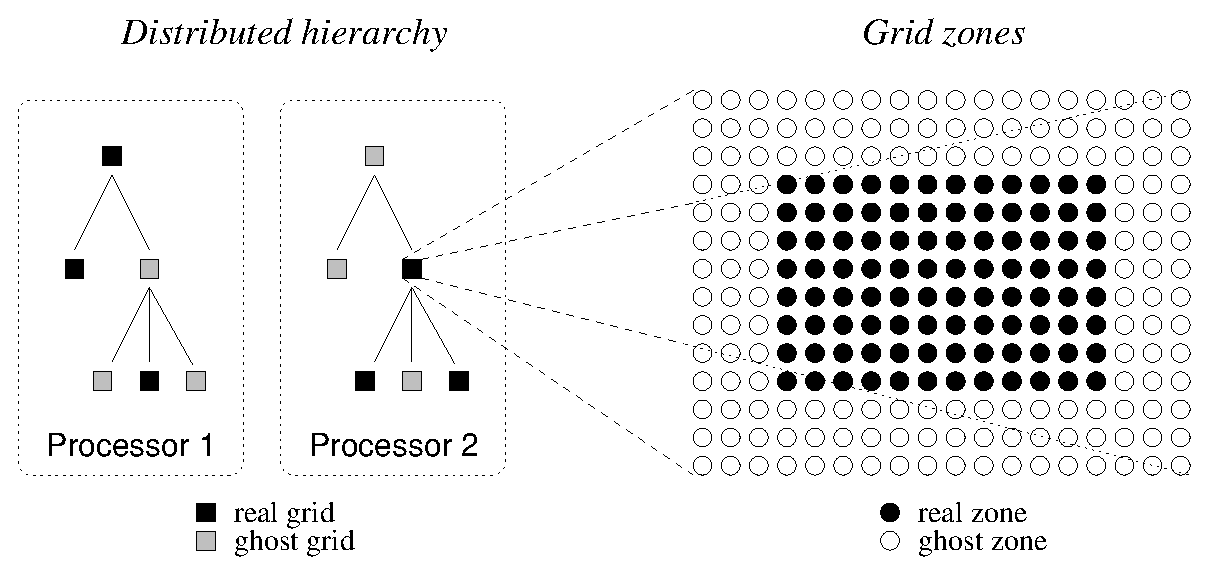
\includegraphics[width=0.5\textwidth]{figures/amr_hierarchy.eps}
\end{center}
\caption{\emph{Left:} Example of a simple, distributed AMR hierarchy
showing real and ghost grids.  \emph{Right:} Example 2D \enzo\ grid
showing real and ghost zones, as needed for the PPM hydro stencil. }
\label{fig.amr_hierarchy}
\end{figure}



% ----------------------------------

\subsection{Performance}
\label{sec.performance}

\subsubsection{Performance Measurement \& Instrumentation}

Because of the wide variety of simulations, methods, and uses of Enzo,
it is difficult to state in general terms which routines within the
code will be most costly during a given simulation.  As such, we have
designed a lightweight registering system that has been implemented
for the most commonly used routines (such as the hydrodynamic and
gravity solvers) as well as refinement level timers that measure the
time spent on each level.  Beyond this minimal set of routines, we
have designed a simple way for the user to modify the source by adding
\texttt{TIMER\_START(``Your_Routine_Name'')} and
\texttt{TIMER\_END(``Your_Routine_Name'')}.  These timers are created
and managed individually on each processor in an asynchronous fashion,
and contribute minimal computational, memory, and IO overhead.

At each complete root grid time step (or less often if specified),
each timer is then communicated to the root processor where it
calculates the mean, standard deviation, minimum, and maximum for each
of the timers across all processors.  For level timers, there are additional
attributes such as the number of cell updates, the current number of
grids, and the average cells/s/MPI process.  This information is then
output to a logfile.  This provides a simplified interface to the user
that can be used to diagnose performance issues as well as estimate a
given problem type's scalability.  In addition to the logfile, we have
developed a plotting interface for quickly producing figures that
process the data from the logfile.  These capabilities are described
in the online documentation, along with a further discussion of the
performance measurement implementation.

\subsubsection{Unigrid scaling}
\label{sec:weak_scaling}

\begin{figure}
\begin{center}
\includegraphics[width=0.6\textwidth]{figures/enzo_unigrid_weak_scaling.eps}
\caption{\enzo\ weak scaling performance for a set of Lyman alpha
forest cosmology simulations with constant comoving spatial resolution
per grid cell, showing cell updates per second per computational core
plotted as a function of the number of root grid tiles of dimension
$128^3$ (R) in each dimension.  The number of MPI tasks is N$ = R^3$,
so R$ = 16$ on this plot corresponds to a $2048^3$ computational mesh
running on 4,096 MPI tasks.  This plot goes from R$ = 2$ (8 MPI tasks)
to R$ = 24$ (13,824 MPI tasks) on two supercomputers -- NICS Kraken
and ORNL Jaguar when they were Cray XT4 systems -- and using 1, 2 or 4
MPI processes per node, where each compute node contained a single
quad-core AMD Opteron CPU having a speed of 2.1 GHz on Jaguar and 2.3
GHz on Kraken.}
\label{fig.uniscale}
\end{center}
\end{figure}

It is advantageous to use \enzo\ in its ``unigrid'' (i.e.,
non-adaptive mesh) mode for a variety of problems, including
non-gravitating turbulence
\citep[e.g.,][]{2002ApJ...569L.127K,Kritsuk04}, the Lyman-alpha forest
\citep{2005MNRAS.361...70J,2009MNRAS.399.1934P}, or feedback of
metal-enriched gas from galaxies into the intergalactic medium
\citep{2004ApJ...601L.115N,2011ApJ...731....6S}.  Achieving good
scaling of the code in unigrid mode is relatively straightforward --
upon initialization, unigrid simulations are decomposed such that each
MPI process has a roughly equal subvolume (and thus number of grid
cells), meaning that work is evenly distributed.  Communication
patterns for both the gravity solve (which uses a fast Fourier
transform) and the fluid solves (which transfer boundary information
between subvolumes) are predictable and straightforward, and
rebuilding of the grid hierarchy does not take place, removing a
substantial global operation and a great deal of communication.

Figure~\ref{fig.uniscale} shows \enzo\ weak scaling results for a
sequence of scaled unigrid Lyman alpha forest calculations. These
calculations include dark matter dynamics, hydrodynamics using the
piecewise parabolic method, six-species non-equilibrium chemistry and
radiative cooling, and a uniform metagalactic ultraviolet background.
In this sequence of test calculations, we perform a weak scaling test
on up to 13,824 MPI tasks on the NICS Kraken XT4 and ORNL Jaguar XT4
supercomputers\footnote{These simulations were performed prior to
conversion of both machines to the current-generation systems}.  In
this test, each MPI task was given a $128^3$ root grid tile (i.e.,
$128^3$ grid cells containing baryon quantities) and, initially,
approximately $128^3$ dark matter particles.  The number of grid cells
was constant throughout the calculation; the number of dark matter
particles varies as they are moved from subvolume to subvolume as
structure evolves.  The grid resolution was kept at a constant
comoving size of $\simeq 40$~kpc/h, and as the core count was
increased, so was the simulation volume.  On each machine, a compute
node contained a single AMD Opteron quad-core chip (2.1 Ghz on Jaguar;
2.3 Ghz on Kraken) with 2 GB/memory per core (8 GB/total per node).
Both machines used the SeaStar2 interconnect.  In the scaling study,
calculations were run with 1, 2, or 4 MPI tasks per node.  The figure
shows cell updates per second per MPI process; perfect scaling would
be a horizontal line.

As can be seen in Figure~\ref{fig.uniscale}, the unigrid weak scaling
performance of the code is extremely good for this problem, with only
a 20\% decrease in cell updates/second/task as the code is scaled from
8 to 4,096 MPI tasks, and a 40\% decrease in performance overall going
from 8 to 13,824 (or $24^3$) MPI tasks.  We speculate that this
decrease is likely to be partially due to global MPI communications
used to, e.g., calculate the overall timestep of the simulation, and
also likely due to load imbalances due to increasing cosmological
power (and thus an increasingly uneven distribution of dark matter
particles between MPI tasks at late times) as the simulation volume
grows.  We also observe that a systematic difference in speed can be
seen between the two machines, which can be attributed primarily to
the slightly faster CPUs on Kraken at th etime (2.3 Ghz, vs. 2.1 Ghz
on Jaguar).  The difference in speed when using different numbers of
MPI tasks per node can be attributed primarily due to differences in
competing usage of shared cache on the quad-core chips used on this
machine.

Broadly, excellent scaling in \enzo's unigrid mode is seen for a
variety of problems as long as each compute core is given an adequate
amount of work to do.  For cosmological simulations, this value has
been empirically determined to be roughly $128^3$ cells per core.  If
fewer cells per core are used, the CPU is essentially data-starved,
and poor scaling is observed due to computing units being idle while
waiting for information to be communicated from other processes (for,
e.g., boundary information or gravity solves).  Substantially larger
cell counts per core would in principle help scaling by reducing the
amount of inter-process communication needed, but larger cell counts
are typically impractical on most machines due to memory limits.

As a final point, we observe that scaling at larger core counts has
been measured, but only with an experimental hybrid-parallel (MPI +
OpenMP) version of \enzo.  Using this version, scaling comparable to
that shown in Figure~\ref{fig.uniscale} was seen on up to 98,304 cores
on the NICS Kraken XT5 (an upgraded version of the XT4 machine used
for the scaling study shown in the figure), using 2-8 OpenMP threads
per MPI process.  Hybrid parallelism has the potential to
substantially improve scaling by reducing the amount of communication
per grid tile (as described in the previous paragraph); however, the
optimal ratio of OpenMP threads per MPI task seems to vary
substantially between computational platforms and astrophysical
problems/required \enzo\ physics modules, and thus we hesitate to
provide strict guidelines here.

\subsubsection{AMR scaling}

\begin{figure}
\begin{center}
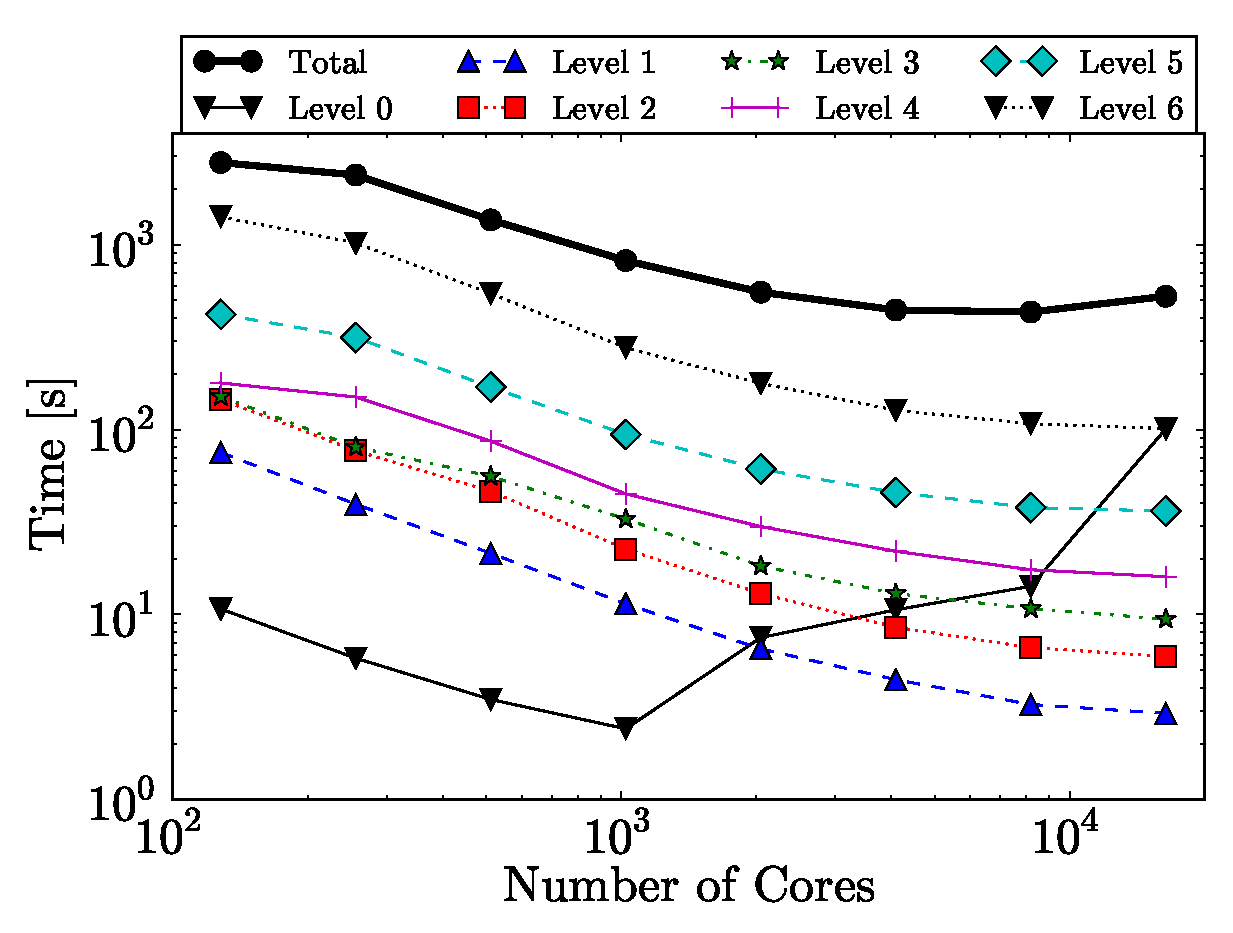
\includegraphics[width=0.48\textwidth]{figures/strong_scaling_levels.eps}
\hfill
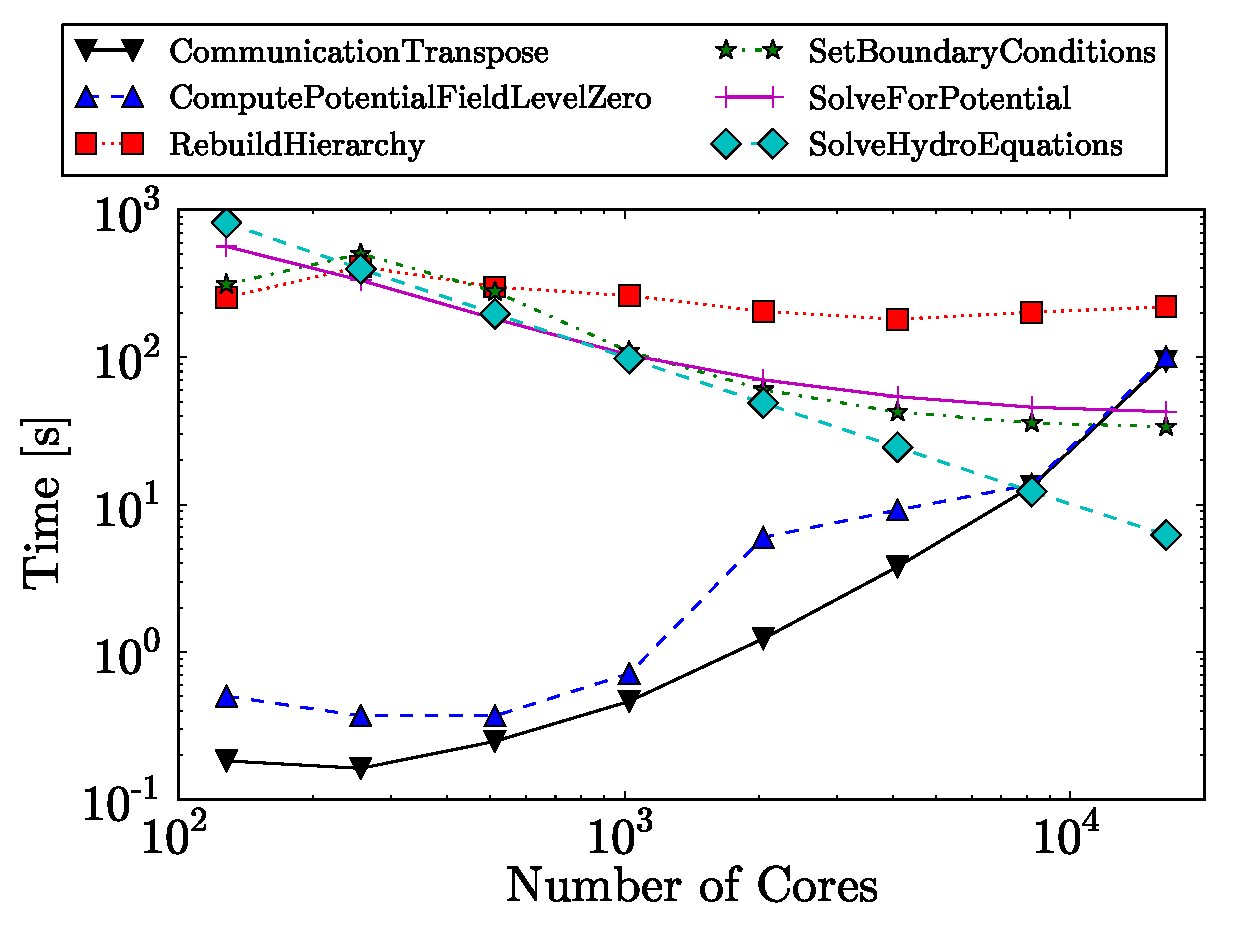
\includegraphics[width=0.48\textwidth]{figures/strong_scaling_routines.eps}
\end{center}
\caption{\emph{Left:} Strong scaling test of a 512$^3$ AMR
cosmological calculation.  The root grid scaling is not representative
of the true strong scaling of Enzo because the root grid tiles are not
repartitioned when a simulation is restarted with additional cores.
The weak scaling test in Figure \ref{fig.uniscale} is more
representative of the scaling on the root level.  The performance in
the refined levels show good strong scaling up to 2,048 cores.
\emph{Right:} Time spent in representative major routines in the same
AMR calculation.}
\label{fig:strong_scaling}
\end{figure}

Many astrophysical problems, such as cosmological galaxy formation
\citep{2012ApJ...749..140H}, high-resolution disk galaxy simulations
\citep{2011ApJ...738...54K}, high-redshift \citep{2009Sci...325..601T}, and present-day
star formation \citep{Collins12a}, involve multi-scale physics that
span several orders of magnitude in both space and time.  In these
situations, using Enzo in its adaptive mesh refinement mode is
beneficial.  Because the adaptive grid hierarchy is dynamic, grid
boundaries and, thus, communication patterns can be unpredictable,
hindering strong scaling behavior to high core counts.

Figure \ref{fig:strong_scaling} shows strong scaling results from a
single 50 Mpc/h cosmology simulation run on $N_{\rm core}$ compute
cores, ranging from 128 to 16,384 cores at power-of-two intervals.  It
was run on the NICS Kraken XT5 supercomputer, which has two AMD
Opteron hexa-core processors with 16 GB of memory per compute node.
The simulations that utilized 128, 256, and 512 cores were executed on
128 nodes because of the memory requirements.  The higher core count
simulations were run with 8 cores per node.  This simulation would not
run with 12 cores per node because of the memory overhead associated
with the grid hierarchy being duplicated on each MPI process.
However, this overhead is greatly diminished if a hybrid-parallel (MPI
+ OpenMP) approach is used.

This simulation includes dark matter dynamics, hydrodynamics using the
piecewise parabolic method, six-species non-equilibrium chemistry and
radiative cooling, and a uniform metagalactic ultraviolet background.
The simulation uses the space-filling curve method for load balancing
the AMR grids.  It has a $512^3$ root grid that is divided into 512
tiles, and 6 additional AMR levels are used.  We perform these scaling
tests when the simulation reaches $z=4$, where the AMR grid hierarchy
is well-developed and is thus a reasonable representation of AMR
simulation behavior in general.  The results shown in Figure
\ref{fig:strong_scaling} come from a single root-level timestep
of $\Delta t = 2.1\, \textrm{Myr}$.  At this time, there are $3.04 \times
10^5$ AMR grids, $9.03 \times 10^8$ ($\sim 967^3$) computational
cells, and $1.34 \times 10^8$ dark matter particles in total.  The
breakdown of the number of AMR grids, cells, timesteps, and number of
cell updates on each level is shown in Table \ref{tab:amr_scale}.

%%%%%%%%%%%%%%%%%%%%%%%%%%%%%%%%%%%%%%%%%%%%%%%%%%%%%%%%%%%%%%%%%%%%%%%%
\begin{table*}
  \begin{center}
  \caption{Strong scaling test computational details}
  \begin{tabular*}{0.9\textwidth}{@{\extracolsep{\fill}}c c c c c}
    \tableline\tableline
    {Level} & {$N_{\rm grid}$} & {$N_{\rm cells}$} & {$N_{\rm up}$} &
    {$N_{\rm timesteps}$}\\
    \tableline
    0 & 512 & $1.34 \times 10^8$ & $1.34 \times 10^8$ & 1\\
    1 & 61,868 & $4.01 \times 10^8$ & $4.01 \times 10^8$ & 1\\
    2 & 91,182 & $1.99 \times 10^8$ & $5.96 \times 10^8$ & 3\\
    3 & 59,932 & $7.62 \times 10^7$ & $5.34 \times 10^8$ & 7\\
    4 & 40,700 & $3.32 \times 10^7$ & $5.65 \times 10^8$ & 17\\
    5 & 28,346 & $2.76 \times 10^7$ & $1.36 \times 10^9$ & 49\\
    6 & 19,771 & $2.80 \times 10^7$ & $5.25 \times 10^9$ & 187\\
    \tableline
    Total & 302,311 & $9.03 \times 10^8$ & $8.83 \times 10^9$ & --\\
  \end{tabular*}
  \parbox[t]{0.9\textwidth}{\textbf{Note.} --- Data shown at $z=4$ for
    a root grid timestep of 2.1~Myr.  
    Col. (1): AMR Level. Col. (2):
    Number of grids. Col. (3): Number of computational
    cells. Col. (4): Number of cell updates. Col. (5): Number of
    timesteps.}
  \label{tab:amr_scale}
  \end{center}
\end{table*}

%%%%%%%%%%%%%%%%%%%%%%%%%%%%%%%%%%%%%%%%%%%%%%%%%%%%%%%%%%%%%%%%%%%%%%%%

The left panel in Figure \ref{fig:strong_scaling} shows the
computational and communication time spent on each level.  In the AMR
levels, there exists good strong scaling up to 2,048 cores, and
marginal speed-ups are found at 4,096 cores.  On the root-grid level,
there exists good scaling up to 1,024 cores, but the performance
dramatically decreases at higher core counts.  This occurs because the
root grid is not re-partitioned into $N_{\rm core}$ tiles when the
simulation is restarted with a different core count.  This feature can
be easily implemented and is planned in the next major release of
Enzo, where scaling results would be similar to the weak scaling shown
in \S\ref{sec:weak_scaling}.  The right panel in Figure
\ref{fig:strong_scaling} shows the time spent in some representative
major routines in Enzo.  The local physics routines, for example
\texttt{SolveHydroEquations}, exhibit perfect strong scaling because
they involve no communication.  By investigating the scaling behavior
in each routine, it is clear that the communication in the
\texttt{SetBoundaryConditions}, \texttt{SolveForPotential} (multi-grid
solver in AMR levels), and \texttt{RebuildHierarchy} are responsible
for the lack of strong scaling at $N_{\rm core} \ga$~4,096 in this
particular simulation.  The transpose of the root grid tiles are
responsible for the performance decrease because it is not optimized
for situations where the number of tiles is greater than the number of
MPI processes.  These results are directly applicable to simulations
with similar computational demands.  In simulations with fewer
computational cells, strong scaling will cease at a smaller core count
because the CPUs will become data-starved more quickly, and the
opposite occurs with larger simulations.


\subsubsection{An Approximate Time and Memory Scaling Model}

In this section, we develop a simple, approximate model to estimate
the computational time and memory required to complete a given
calculation.  Note that we are {\it not} trying to model parallel
performance (which was discussed in the previous section), but have an
even simpler goal: to determine how to scale computational time
estimates as we increase the simulation resolution.  This is a
straightforward thing to do in codes that use static grids, as the
computational effort per time step is constant.  However, for an AMR
calculation, the number of grids that will be generated during the run
is not known in advance, and so the CPU time per problem time can vary
drastically throughout the calculation.  For example, at the beginning
of the simulation when the densities are nearly uniform, only the
static grid is required and the calculation progresses rapidly.
However, as structure forms and dense clumps are generated, the number
of grid points swells by orders of magnitude (an increase of $10^3$ is
not uncommon) and most of the CPU time is consumed at late times.
Therefore, simply performing a few steps at the beginning of the
calculation does produce a good estimate of the required CPU time.

Nevertheless, we can try to determine how the compute time scales for
a given run as we increase the resolution.  First, we neglect
particles and concentrate on the time taken by the grids, which can be
justified both theoretically and empirically\footnote{Since the
potential is calculated on the grid, the only particle costs are:
depositing mass to the grid, interpolating accelerations, and updating
particle positions and velocities.  These are relatively
computationally inexpensive operations.}.  Second, we break the
problem down slightly, and examine the scaling over a short enough
period of time that the grid structure does not change significantly
(i.e. the number of grids at each level remains approximately
constant).  We then assume that the whole run scales in the same way,
or in other words, that changes in the resolution affect the
simulation in the same way at each time step.  This is usually a good
approximation, as the most costly parts of the calculation typically
don't change their characteristics substantially between timesteps.

To make progress, we assume that the computational cost to advance a
single cell by one timestep is a constant.  This can be incorrect if
the chemistry solver requires many iterations, but is usually fairly
accurate.  For a unigrid calculation, the time would by proportional
to $N_{\rm root}^4$ since the number of cells scales as $N_{\rm
root}^3$ and, assuming the Courant condition is the 
factor that controls the time step, the number of steps to advance the
calculation over a given time interval is
proportional to $N_{\rm root}.$ Therefore, to advance a hierarchy a
given time interval, we find, accounting for all levels and using a refinement
factor of 2,
\begin{equation} t_{\rm SU} = C_1 \sum_l f_l N_{\rm root}^4 2^{4l}
\end{equation} where $C_1$ is a constant, which can be thought of as
the time taken to advance a single cell.  The factor $f_l$ is the
fraction of the volume on a given level that is actually refined.  By
definition $f_0 = 1$, and $f_l \le 1$.  In writing down this equation,
we neglect a number of costs that are not directly proportional to
cell count, including communication between processors, the $\log{N}$
factor for the root grid FFT, cache misses, optimizations, and other
costs associated with processing the hierarchy.  The first item on
this list, in particular, is clearly important for large processor
counts; however, we neglect parallel considerations in this section.

Note that unless $f_l/f_{l+1} < 1/16$ (i.e. if less then about 6\% of
a given level is further refined), the cost per level will increase
with level.  A key question, therefore, is the value of $f_l$ for each
level.  Unfortunately, this depends strongly on the simulation being
run.  In Figure~\ref{fig:scaling}, we show the values of $f_l$ for
three simulations: two cosmological runs with varying box size, and a
third simulation focusing on a single disk galaxy.

\begin{figure}
\centerline{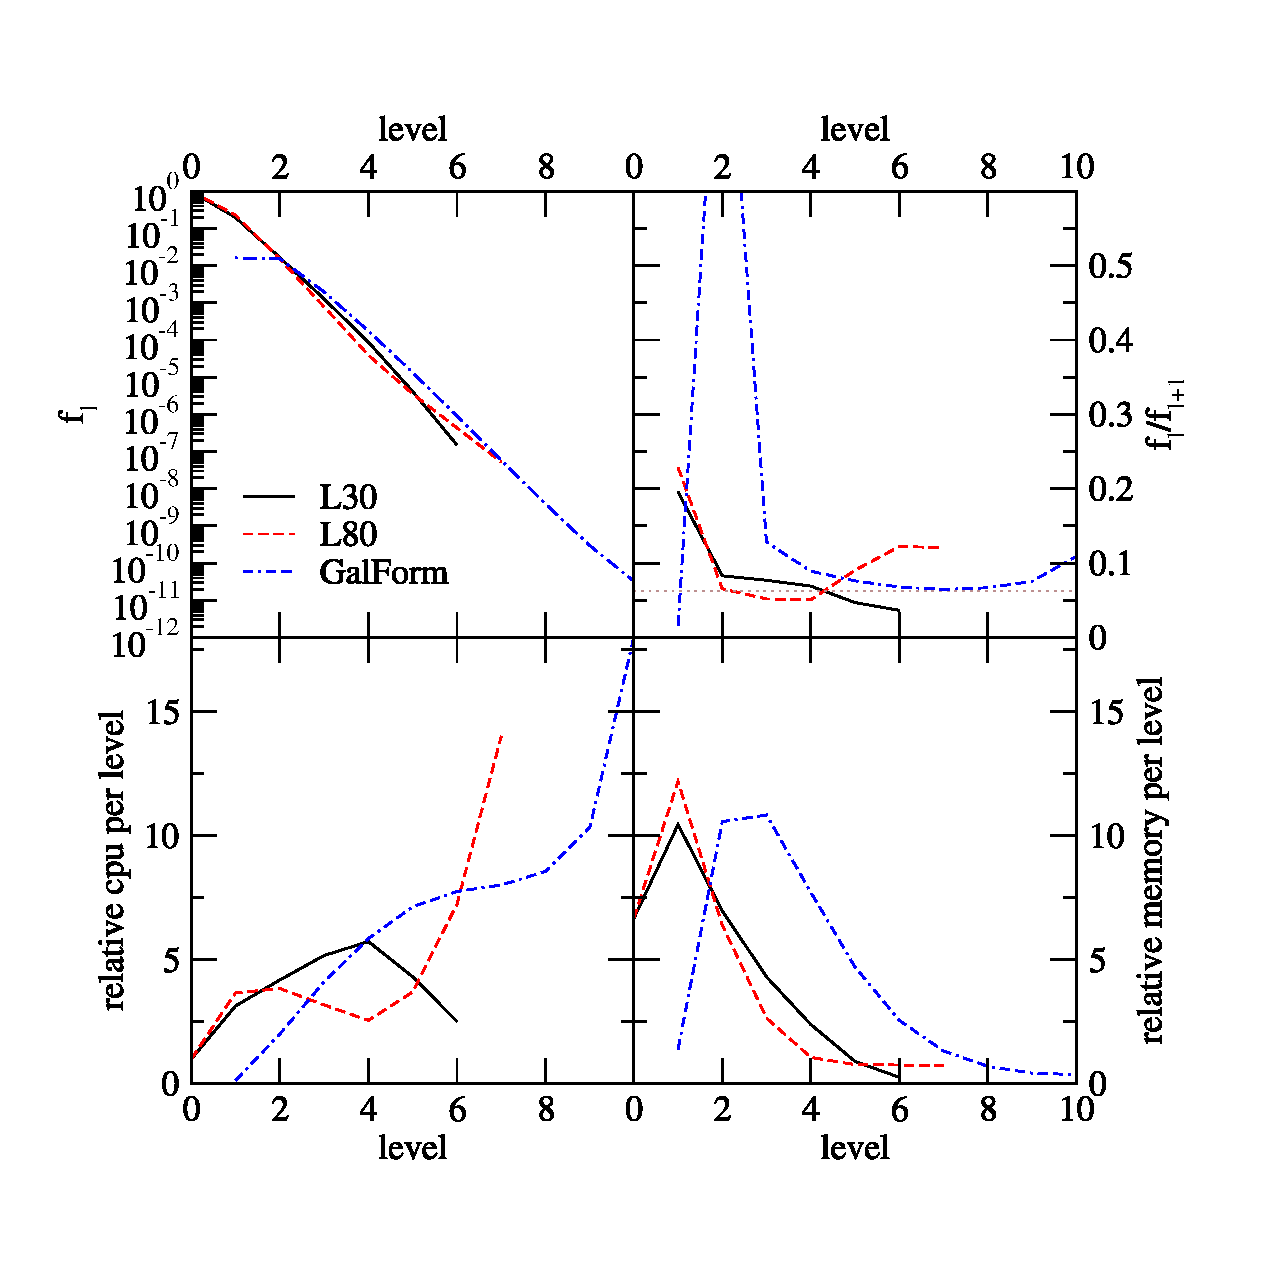
\includegraphics[width=0.7\textwidth]{figures/scaling_plot2}}
\caption{This figure show (clockwise from upper left), the covering
fraction $f_l$ of the grids on a given level $l$, the ratio of
$f_{l}/f_{l+1}$, the relative memory usage of each level (normalized
by the memory usage of level 0), and, in the lower-left panel, the
relative CPU usage of each level, again normalized by $l=0$.  In each
panel, three curves are shown: the solid black and long dashed red are
two cosmological simulations with box sizes of 30 h$^{-1}$ Mpc and
80h$^{-1}$ Mpc respectively.  The dot-dashed blue line is for a
non-cosmological simulation of a ram-pressure stripped galaxy.  In the
top-right panel, there is a line at the critical ratio of 0.06, which
determines if the next finer level ($l+1)$ takes more (above) or less
(below) CPU time than level $l$.}
\label{fig:scaling}
\end{figure}

As, the figure demonstrates, the $f_l$ values all show a sharp decline
with level, dropping as power-laws with the level $l$.  Focusing first
on the ``refine-everywhere" cosmological runs, which both show similar
behavior despite the different box sizes and redshifts at which we
collect the data.  In fact, we find these results are very typical for
cosmological runs, with only slight variations depending on the exact
system that is being simulated.  The top-left panel
shows the ratio of $f_{l}/f_{l+1}$ which, remarkably, hovers around
the critical value of 0.0625 determined earlier.  This implies that
the relative CPU usage of each level, shown in the lower-left panel,
is nearly flat, and that going to additional levels of refinement only
increases the amount of calculation by a factor of roughly $1/l_{\rm
max}$.  Even in the most extreme case, the L80 run, the last level
adds only 25\% to the computation time.

The memory used by each level, on the other hand, scales as
\begin{equation}
{\rm memory} = C_2 \sum_l f_l N_{\rm root}^3 2^{3l}
\end{equation}
and the terms in this sum are shown in the bottom-right panel of
Figure~\ref{fig:scaling}.  This demonstrates that the memory usage is
dominated by the top three levels, and adding additional levels only
adds minimally to the memory usage of the run.  We have empirically
tested this scaling for cosmological simulations and found it to be
reasonably accurate (although the increase is typically slightly
larger than found here, usually 30-50\%, probably because of
less-than-ideal parallel scaling).

The physical reason for the $f_{l+1}/f_l$ ratios found in the
cosmological simulations appears to be due to a combination of the
density structure of individual clouds, and the distribution of the
clouds themselves.  In particular, we note that for a $\rho \propto
r^{-2}$ density profile, the Lagrangian refinement criteria typically used in
such simulations produces an $f_{l+1}/f_l$ ratio of 1/8 for a single,
resolved cloud.  Of course, at some point we would resolve the flat
density of individual clouds and the ratio would climb, making further
refinement more costly; however, we are not yet in this regime in this
example.

These conclusions are, however, highly dependent on the type of run
being performed.  We contrast this cosmological case to the simulation
of a galaxy formation run, as shown by the dot-dashed curves in
Figure~\ref{fig:scaling}.  Note that grid levels 1 and 2 in this simulation are statically
refined to ensure that the Lagrangian volume of the galaxy halo is resolved
to at least level 2 at all times. More importantly, the
$f_{l+1}/f_{l}$ ratio of the highest levels are systematically
slightly larger than the critical 0.0625 value, indicating that the
CPU time is dominated by the most refined levels, as shown in the
bottom-left panel.  The memory usage is dominated by levels 2 and 3,
the static levels, as the bottom-right panel demonstrates.  In this
case, adding more levels of refinement would somewhat increase the
cost of the simulation.

We have focused thus far on scaling when increasing $l_{\rm max}$, but
without changing the refinement criteria.  However, we can also keep
the levels fixed and modify the refinement criteria.  For cosmological
runs, this is typically done by increasing the mass resolution (and
simultaneously decreasing the dark matter particle mass), and adding
additional linear small-scale modes to the initial conditions.  The
effect of this is to boost the $f_l$ values at all levels (except for
the root grid where $f_0$ is already 1) by a factor linearly
proportional to the increase in the mass resolution.  This is because
the refinement criteria typically boosts the number of refined cells
on the first and subsequent levels by this factor.  Again, we have
empirically demonstrated that this scaling is approximately valid,
provided that we keep the maximum level constant.

Putting this together, we find an approximate scaling for the
computational time required for cosmological simulations:
\begin{equation}
t_{\rm SU} \propto M_{\rm res}^{-1} l_{\rm max}.
\end{equation}
This is approximately accurate, and gives users some way to estimate
compute times for \enzo\ calculations.  